%%%%%%%%%%%%%%%%%%%%%%%%%%%%%%%%%%%%%%%%%%%%%%%%%%%%%%%%%%%%%%%%%%%%%%%%%%%%%%%
\chapter{Probabilidad y distribuciones}
%%%%%%%%%%%%%%%%%%%%%%%%%%%%%%%%%%%%%%%%%%%%%%%%%%%%%%%%%%%%%%%%%%%%%%%%%%%%%%%

Los conceptos de aleatoriedad y probabilidad son fundamentales para las
estadísticas. Es un hecho empírico que la mayoría de los experimentos e
investigaciones no son perfectamente reproducibles. El grado de
irreproducibilidad puede variar: Algunos experimentos en física pueden producir
datos que son exactos hasta muchos decimales, mientras que los datos sobre
sistemas biológicos son típicamente mucho menos confiables. Sin embargo, la
visión de los datos como algo que proviene de una distribución estadística es
vital para entender los métodos estadísticos. En esta sección se esbozan las
ideas básicas de probabilidad y las funciones que tiene \textbf{R} para el
muestreo aleatorio y el manejo de las distribuciones teóricas.

%%%%%%%%%%%%%%%%%%%%%%%%%%%%%%%%%%%%%%%%%%%%%%%%%%%%%%%%%%%%%%%%%%%%%%%%%%%%%%%
\section{Muestreo aleatorio}
%%%%%%%%%%%%%%%%%%%%%%%%%%%%%%%%%%%%%%%%%%%%%%%%%%%%%%%%%%%%%%%%%%%%%%%%%%%%%%%

Gran parte de los primeros trabajos en la teoría de la probabilidad se referían
a juegos y apuestas, basados en consideraciones de simetría. Por lo tanto, la
noción básica de una  muestra aleatoria es la de repartir de una baraja bien
barajada o recoger bolas numeradas de una urna bien revuelta.

En \textbf{R}, se pueden simular estas situaciones con la función
\texttt{sample}. Si quieres elegir cinco números al azar del conjunto de
\texttt{1:40}, entonces se puede escribir:

\begin{lstlisting}[language=R]
> sample(1:40,5)
[1] 36 37 26 24  3
\end{lstlisting}

El primer parámetro (\texttt{x}) es el vector de valores posibles de dónde
obtendremos la muestra y el segundo (\texttt{size}) es el tamaño de la muestra.
En realidad, \texttt{sampe(40,5)} sería suficiente ya que un solo número se
interpreta como la longitud de una secuencia de números enteros desde el 1.

Note que el comportamiento predeterminado de \texttt{sample} es el de
\textit{muestreo sin reemplazo}. Es decir, las muestras no contendrán ningún
número repetido, y \texttt{size} obviamente no puede ser mayor que la longitud
del vector a muestrear. Si quiere muestreo con reemplazo, entonces necesita
agregar el parámetro \texttt{replace=TRUE}.

El muestreo con reemplazo es adecuado para modelar lanzamientos de monedas o
lanzamientos de un dado. Así, por ejemplo, para simular 10 lanzamientos de
monedas podríamos escribir:

\begin{lstlisting}[language=R]
> sample(c("H","T"), 10, replace=T)
[1] "T" "T" "T" "T" "T" "H" "H" "T" "H" "T"
\end{lstlisting}

En un lanzamiento normal de monedas, la probabilidad de cara debe ser igual a la
probabilidad de cruz, pero la idea de un evento aleatorio no se limita a casos
simétricos.  Podría aplicarse igualmente bien a otros casos, como el resultado
exitoso de un procedimiento quirúrgico. Esperemos que haya más de un 50\% de
posibilidades de que esto suceda. Puede simular datos con probabilidades no
simétricas para los resultados (por ejemplo, un 90\% de probabilidad de éxito)
usando el parámetro \texttt{prob} de \texttt{sample}, como ser:

\begin{lstlisting}[language=R]
> sample(c("succ", "fail"), 10, replace=T, prob=c(0.9, 0.1))
[1] "succ" "succ" "succ" "succ" "succ" "succ" "succ" "succ"
[9] "succ" "succ"
\end{lstlisting}

Sin embargo, esta puede no ser la mejor manera de generar una muestra de este
tipo. Ver la discusión posterior de la distribución binomial.

%%%%%%%%%%%%%%%%%%%%%%%%%%%%%%%%%%%%%%%%%%%%%%%%%%%%%%%%%%%%%%%%%%%%%%%%%%%%%%%
\section{Cálculos de probabilidad y combinatoria}
%%%%%%%%%%%%%%%%%%%%%%%%%%%%%%%%%%%%%%%%%%%%%%%%%%%%%%%%%%%%%%%%%%%%%%%%%%%%%%%

Volvamos al caso del muestreo sin reemplazo, específicamente
\texttt{sample(1:40,5)}. La probabilidad de obtener un número dado como ser, el
primero de la muestra debe ser de $1/40$, la del siguiente es de $1/39$, y así
sucesivamente. La probabilidad entonces  de obtener una determinada combinación
de 5 números,  debe ser de $1/(40 \times 39 \times 38 \times 37 \times 36)$.  En
\textbf{R}, puede utilizar la función \texttt{prod}, para calcular el producto
de un vector de números:

\begin{lstlisting}[language=R]
> 1/prod(40:36)
[1] 1.266449e-08
\end{lstlisting}

Sin embargo, tenga en cuenta que esta es la probabilidad de que se den los
números en un orden determinado. Si se tratara de un juego como el de la
lotería, entonces preferiría estar interesado en la probabilidad de adivinar
correctamente un determinado conjunto de cinco números.  Por lo tanto, también
es necesario incluir los casos que dan los mismos números pero en un orden
diferente.  Puesto que obviamente la probabilidad de cada caso va a ser la
misma, todo lo que tenemos que hacer es averiguar cuántos casos de este tipo hay
y multiplicarlos por eso. Hay cinco posibilidades para el primer número, y para
cada uno de ellos hay cuatro posibilidades para el segundo, y así sucesivamente;
es decir, el número es $5 \times 4 \times 3 \times 2 \times 1$. ¡Este número
también se escribe como $5!$ (factorial de 5)!. Así que la probabilidad de un
cupón ganador de la lotería, sería:

\begin{lstlisting}[language=R]
> prod(5:1)/prod(40:36)
[1] 1.519738e-06
\end{lstlisting}

\newpage

Hay otra forma de llegar al mismo resultado. Note que como el conjunto real de
números es irrelevante, todos los conjuntos de cinco números deben tener la
misma probabilidad. Así que todo lo que tenemos que hacer es calcular el número
de maneras de elegir 5 números de un total de 40. Esto se puede definir como:

\begin{gather*}
\left(
    \begin{array}{c}
      40\\
      5
  \end{array}
\right) = \frac{40!}{5!35!} = 658008
\end{gather*}

\begin{tradnote}
    Hay 658008 posibles combinaciones de 5 numéros, la posibilidad de elegir la
    combinación ganadora, es obviamente:

    \begin{gather*}
    \frac{1}{658008} = 1.519738e-06
    \end{gather*}

\end{tradnote}

En \textbf{R}, se puede utilizar la función \texttt{choose} para calcular este
número, y por lo tanto la probabilidad es:

\begin{lstlisting}[language=R]
> 1/choose(40,5)
[1] 1.519738e-06
\end{lstlisting}

%%%%%%%%%%%%%%%%%%%%%%%%%%%%%%%%%%%%%%%%%%%%%%%%%%%%%%%%%%%%%%%%%%%%%%%%%%%%%%%
\section{Distribuciones discretas}
%%%%%%%%%%%%%%%%%%%%%%%%%%%%%%%%%%%%%%%%%%%%%%%%%%%%%%%%%%%%%%%%%%%%%%%%%%%%%%%

Al examinar las repeticiones independientes de un experimento binario, normalmente
no nos interesaría saber si cada caso es un éxito o un fracaso, sino más bien el
número total de éxitos (o fracasos). Obviamente, este número es aleatorio ya que
depende de los resultados aleatorios individuales, y por lo tanto se le llama
\textit{variable aleatoria}. En este caso, es una \textit{variable
aleatoria} de valor discreto que puede tomar valores 0, 1, .... \textit{n},
donde \textit{n} es el número de repeticiones. Las variables aleatorias continuas se
verán más tarde.


Una variable aleatoria \textit{X} tiene una \textit{distribución de
probabilidad} que puede describirse utilizando \textit{probabilidades puntuales}
\textit{f(x) = P(X = x)}  o la \textit{función de distribución acumulativa F(x)
= P(X <= x)}. En el caso que nos ocupa, la distribución puede ser elaborada
como si tuviera las probabilidades puntuales

\begingroup
\Large
\begin{gather*}
    f(x) = \binom{n}{x} p^{x}(1-p)^{n-x}
\end{gather*}
\endgroup

Esto se conoce como \textit{distribución binomial}, y $\binom{n}{x}$ se los
llama \textit{coeficientes binomiales}. El parámetro \textit{p} es la
probabilidad de un resultado exitoso en una prueba individual. Una gráfica de
las probabilidades puntuales de la distribución binomial aparece más adelante en
la Figura 3.2.

Retrasamos la descripción de las funciones de \textbf{R} relacionadas con la
distribución binomial hasta que hayamos discutido distribuciones continuas, para
que podamos presentar las convenciones de forma manera unificada

Muchas otras distribuciones pueden derivarse de los modelos de probabilidad
simple. Por ejemplo, la \textit{distribución geométrica} es similar al binomial
pero registra el número de fracasos que ocurren antes del primer éxito

%%%%%%%%%%%%%%%%%%%%%%%%%%%%%%%%%%%%%%%%%%%%%%%%%%%%%%%%%%%%%%%%%%%%%%%%%%%%%%%
\section{Distribuciones continuas}
%%%%%%%%%%%%%%%%%%%%%%%%%%%%%%%%%%%%%%%%%%%%%%%%%%%%%%%%%%%%%%%%%%%%%%%%%%%%%%%

Algunos datos surgen de mediciones en una escala esencialmente continua, por
ejemplo: temperatura, concentraciones, etc. En la práctica, se
registrarán con una precisión finita, pero es útil ignorar esto en el modelado.
Estas mediciones generalmente tendrán un componente de variación aleatoria, lo
que las hace no perfectamente reproducibles. Sin embargo, estas
fluctuaciones aleatorias tenderán a seguir ciertos patrones; normalmente se agruparán en
torno a un valor central, las desviaciones grandes serán más raras que las más
pequeñas.


Para modelar datos continuos, necesitamos definir variables aleatorias cuyo
valor pueda ser cualquier número real. Porque hay infinitos números
infinitamente cerca, la probabilidad de cualquier valor particular será cero,
por lo que no existe una probabilidad puntual como ocurre con los valores
aleatorios discretos. En cambio, tenemos el concepto de \textit{densidad}. Esta
es la probabilidad infinitesimal de acertar una pequeña región alrededor de
textit{x} dividida por el tamaño de la región. La función de la distribución acumulativa
se puede definir como antes, y tenemos la relación

\begingroup
\Large
\begin{gather*}
    f(x) =\int_{x}^{\infty}f(x)dx
\end{gather*}
\endgroup

Hay una serie de distribuciones estándar que surgen en la teoría estadística y
están disponibles en R. Tiene poco sentido describirlos en detalle  aquí excepto
por un par de ejemplos.

La \textit{distribución uniforme} tiene una densidad constante en un intervalo
especificado. (por defecto [0, 1]).

La \textit{distribución normal}  (también conocida como \textit{gaussiana}) tiene
densidad

\begingroup
\Large
\begin{gather*}
    f(x) = -\frac{1}{\sqrt{2\pi}\sigma}exp\left(-\frac{(x-\mu )^2}{2\sigma^2}\right)
\end{gather*}
\endgroup

que depende de su media $\sigma$ y la desviación estándar $\mu$. La distribución
normal tiene un forma característica de campana (Figura 3.1), y modificar
$\sigma$ y $\mu$ simplemente traslada y Amplía la distribución. Es un bloque de
construcción estándar en modelos estadísticos, donde se usa comúnmente para
describir la variación del error. También aparece como una distribución
aproximada en varios contextos; por ejemplo, la distribución binomial para
muestras de gran tamaño puede aproximarse bien mediante por una distribución
normal adecuadamente escalada.

%%%%%%%%%%%%%%%%%%%%%%%%%%%%%%%%%%%%%%%%%%%%%%%%%%%%%%%%%%%%%%%%%%%%%%%%%%%%%%%
\section{Distribuciones incorporadas en \textbf{R}}
%%%%%%%%%%%%%%%%%%%%%%%%%%%%%%%%%%%%%%%%%%%%%%%%%%%%%%%%%%%%%%%%%%%%%%%%%%%%%%%

Las distribuciones estándar que aparecen en relación con la construcción de
modelos y Las pruebas estadísticas se han incorporado a \textbf{R} y, por lo
tanto, puede reemplazar por completo tablas estadísticas tradicionales. Aquí
solo miramos la distribución normal y la distribución binomial, pero otras
distribuciones siguen exactamente el mismo patrón

Se pueden calcular cuatro elementos fundamentales para una distribución
estadística:


\begin{itemize}

    \item
    Densidad o probabilidad puntual

    \item
    probabilidad acumulada, función de distribución

    \item
    Cuantiles

    \item
    Numeros pseudo-aleatorios


\end{itemize}

Para todas las distribuciones implementadas en \textbf{R}, existe una función
para cada uno de los cuatro elementos enumerados anteriormente. Por ejemplo,
para la distribución normal, estas son \texttt{dnorm}, \texttt{pnorm},
\texttt{qnorm} y \texttt{rnorm} (\textit{d}ensidad, \textit{p}robabilidad,
\textit{q}uantil y \textit{r}random, respectivamente).

\subsection{Densidades}

La densidad para una distribución continua es una medida de la relativa
probabilidad de ``obtener un valor cercano a x''. La probabilidad de obtener un
valor en un intervalo particular es el área debajo de la parte correspondiente
de la curva.

\newpage

\begin{figure}[H]
    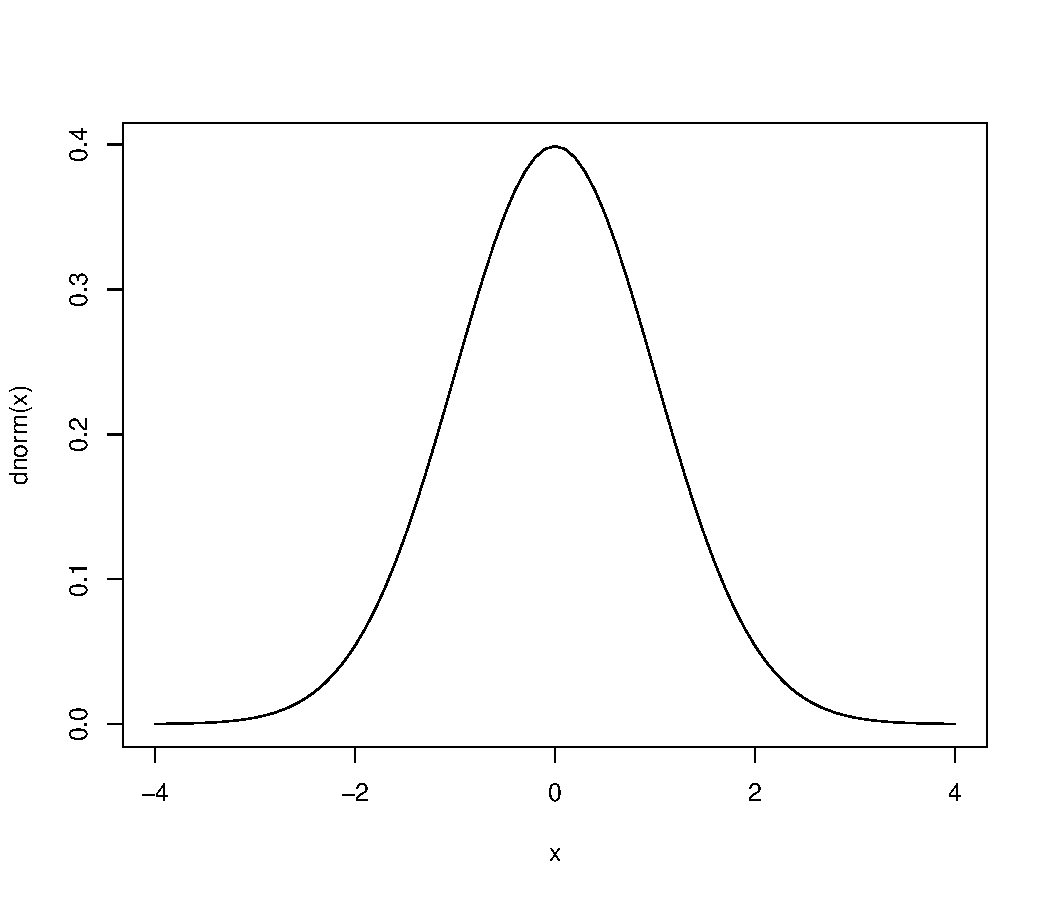
\includegraphics[width=\linewidth]{img/fig-7.pdf}
    \caption{Densidad de la distribución normal}
    \label{fig:fig-7}
\end{figure}

% pdf('doc/fig-7.pdf', height = 6, width = 7)
% x <- seq(-4,4,0.1)
% plot(x,dnorm(x),type="l")
% dev.off()

La función de densidad es probablemente uno de los cuatro tipos de función que
menos e usa en la práctica, pero si, por ejemplo, se desea dibujar la curva de
campana bien conocida de la distribución normal, entonces se puede hacer así:

\begin{lstlisting}[language=R]
> x <- seq(-4,4,0.1)
> plot(x,dnorm(x),type="l")
\end{lstlisting}

(note que es la letra \texttt{'l'} y no el digito \texttt{'1'})

La función \texttt{seq} (\hyperlink{seq}{ver}) se usa para generar valores equidistantes,
aquí de -4 a 4 en pasos de 0.1; es decir, (-4.0, -3.9, -3.8, ... , 3.9, 4.0). los
useof \texttt{type = "l"} como argumento para \texttt{plot} hace que la función
dibuje líneas entre puntos en lugar de trazar los puntos en sí

Una forma alternativa de crear la gráfica es usar \texttt{curve} de la
siguiente forma:

\begin{lstlisting}[language=R]
> curve(dnorm(x), from=-4, to=4)
\end{lstlisting}

Esta es a menudo una forma más conveniente de construir los gráficos, pero
requiere que los valores de \textit{y} se pueden expresar como una función de
\textit{x}.

Para distribuciones discretas, donde las variables solo pueden tomar valores
distintos, Es preferible dibujar un diagrama tipo histograma, aquí para una
distribución binomial con \textit{n} = 50 y \textit{p} = 0,33 (figura
\ref{fig-8})

\begin{lstlisting}[language=R]
x <- 0:50
plot(x,dbinom(x,size=50,prob=.33),type="h")
\end{lstlisting}

\begin{figure}[H]
    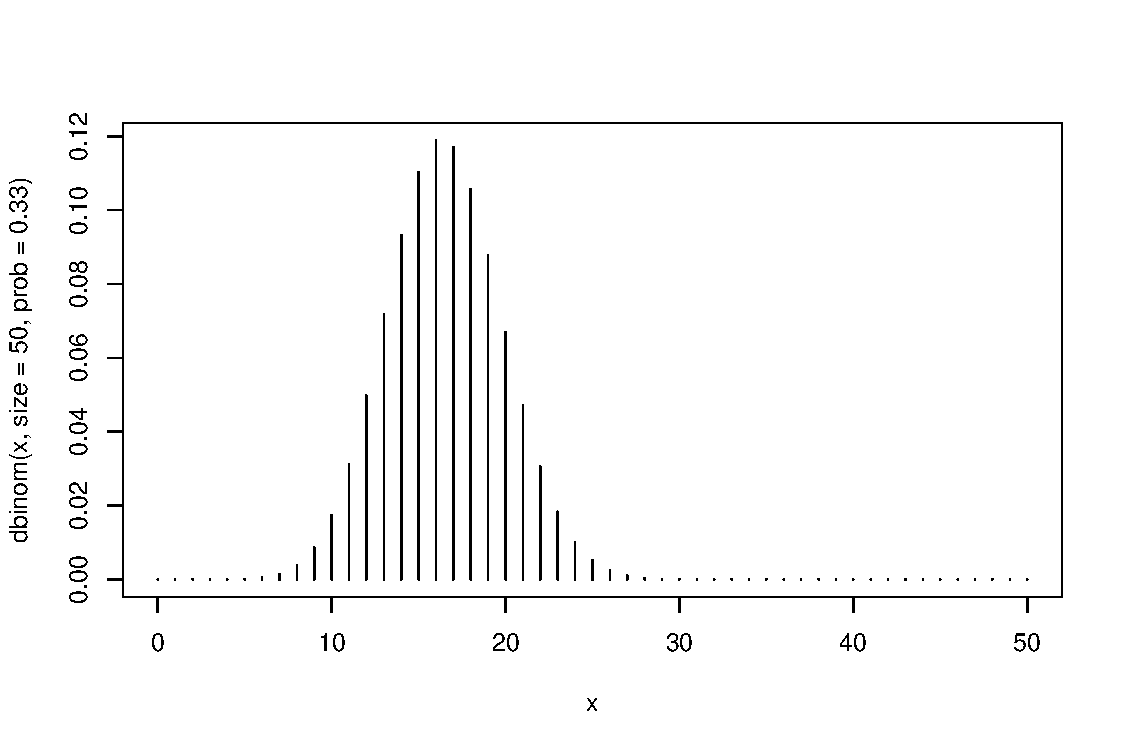
\includegraphics[width=\linewidth]{img/fig-8.pdf}
    \caption{Probabilidades puntuales en binom(50, 0.33)}
    \label{fig-8}
\end{figure}

Tenga en cuenta que esta vez hay tres parámetros en la "función d". Además de
\textit{x}, debemos especificar el número de intentos \textit{y} y la
probabilidad \textit{p}. La distribución dibujada, corresponde, por ejemplo, al
número de cincos o seis en 50 tiradas de un dado simétrico. En realidad,
\texttt{dnorm} también toma más de un parámetro, a saber, la media y la
desviación estándar, pero tienen valores predeterminados de 0 y 1,
respectivamente, ya que lo más frecuente es pedir una distribución normal
estándar.

La expresión \texttt{0:50} es una forma abreviada de \texttt{seq(0, 50, 1)}, es
decir, un vector de número de 0 a 50 (ver \hyperlink{seq}{\texttt{seq}}). Con
\texttt{type  = "h"} indicamos una gráfica tipo histograma.


\subsection{Funciones de distribución acumulativa}

La función de distribución acumulativa describe la probabilidad de "acertar"
\textit{x} o menos en una distribución dada. Las funciones \textbf{R}
correspondientes comienzan con una 'p' (de probabilidad) por convención.

Del mismo modo que se puede trazar densidades, por supuesto, también se puede
dibujar funciones de distribución, pero eso generalmente no es muy informativo.
A menudo, se desean números reales. Digamos que se sabe que alguna medida
bioquímica en individuos sanos está bien descripta por una distribución normal.
con una media de 132 y una desviación estándar de 13. Entonces, si un paciente
tiene un valor de 160, hay


\begin{lstlisting}[language=R]
1 - pnorm(160, mean = 132, sd = 13)
[1] 0.01562612
\end{lstlisting}

es decir, que solo alrededor del 1.5\% de la población en general, tiene ese
valor o más. La función \texttt{pnorm} devuelve la probabilidad de obtener un
valor más pequeño que el primer parámetro en una distribución normal con la
media y la desviación estándar dadas.

Otra aplicación típica es aquella que se relaciona con la pruebas estadísticas.
Considere una prueba sencilla: veinte pacientes reciben dos tratamientos cada
uno (a ciegas y en orden aleatorio) y luego se preguntó si el tratamiento A o B
funcionó mejor. Resultó que a 16 pacientes les gustó más el A. La pregunta es
entonces si esto puede tomarse como evidencia suficiente de que A en realidad es
mejor tratamiento o si en realidad, el resultado podría haber ocurrido por
simple casualidad incluso si Los tratamientos fueron igualmente buenos. Si no
hubiera diferencia entre los dos tratamientos, entonces esperaríamos el número
de personas que favorecen el tratamiento A estar distribuido binomialmente con
\textit{p} = 0.5 y \textit{n} = 20. ¿Que tan (im)probable sería entonces obtener
lo que hemos observado? Como en la distribución normal, necesitamos una
probabilidad de cola, y la suposición inmediata podría ser mirar:


\begin{lstlisting}[language=R]
    1 - pbinom(16, size = 20, prob = .5)
    [1] 0.9987116
\end{lstlisting}

y restarlo de 1 para obtener la cola superior, ¡pero esto sería un error! Lo qué
necesitamos es la probabilidad \textit{del valor observado o uno más extremo}, y
\texttt{pbinom} nos está dando la probabilidad de 16 o menos. Necesitamos usar
"15 o menos" en su lugar

\begin{lstlisting}[language=R]
    > 1-pbinom(15, size = 20, prob =.5)
    [1] 0.005908966
\end{lstlisting}

Si buscamos prueba de dos colas porque no se tiene una idea previa sobre qué
tratamiento es mejor, entonces se deberá agregar la probabilidad de obtener
resultados igualmente extremos en la dirección opuesta. En el caso presente,
esto significa la probabilidad de que 4 o menos personas prefieran el tratamiento A, lo
que da una probabilidad debajo

\begin{lstlisting}[language=R]
    > 1 - pbinom(15, 20, .5) + pbinom(4, 20, .5)
    [1] 0.01181793
\end{lstlisting}

(que obviamente es exactamente el doble de la probabilidad de una sola cola).

Como se puede ver en el último comando, no es estrictamente necesario utilizar
el las palabras claves \textit{size} y \textit{prob} siempre que los parámetros
se den en orden (correspondencia posicional; ver \ref{funparams}).

%%%%%%%%%%%%%%%%%%%%%%%%%%%%%%%%%%%%%%%%%%%%%%%%%%%%%%%%%%%%%%%%%%%%%%%%%%%%%%%
\subsection{Cuantiles}
%%%%%%%%%%%%%%%%%%%%%%%%%%%%%%%%%%%%%%%%%%%%%%%%%%%%%%%%%%%%%%%%%%%%%%%%%%%%%%%

La función cuantil es la inversa de la función de distribución acumulativa. El
\textit{p}-cuantil es el valor con la propiedad de que hay una probabilidad
\textit{p} de obtener un valor menor o igual a él. La mediana es, por
definición, el cuantil del 50 \%.

Algunos detalles sobre la definición en el caso de una distribución discontinua
se pasan por alto aquí. Puedes deducir fácilmente el comportamiento
experimentando con las funciones \textbf{R}.

Las tablas de distribuciones estadísticas casi siempre se dan en términos de
cuantiles. Para un conjunto fijo de probabilidades, la tabla muestra el límite que un
prueba estadística debe cruzar para ser considerada significativa a ese nivel.
Esto es puramente por razones operativas; es casi superfluo cuando tienes
La opción de calcular \textit{p} exactamente.

Los cuantiles teóricos se usan comúnmente para el cálculo de los intervalos de
confianza y para cálculos de potencia en relación con el diseño y dimensionado
de experimentos (ver Capítulo \ref{power_lenght}. Un simple ejemplo de un
intervalo de confianza puede ver aquí (ver también el Capítulo
\ref{datosavanzados})

Si tenemos un número \textit{n} de observaciones normalmente distribuidas con la
misma media $\mu$ y una desviación estándar $\sigma$, es sabido que el promedio
$\bar{x}$ está normalmente distribuido alrededor de $\mu$ con una desviación
estándar $\sigma/\sqrt{n}$. Un intervalode confianza del 95 \% para  $\mu$ puede
obtenerse así:

\begingroup
\Large
\begin{gather*}
    \bar{x} + \sigma/\sqrt{n}\times N _{0.025} \leq \mu \leq \bar{x} +\sigma / \sqrt{n} \times N _{0.975}
\end{gather*}
\endgroup

dónde $N _{0.025}$ es el cuantil 2.5\% en la distribución normal. Si $\sigma =
12$ y hemos medido $n = 5$ personas y encontrado un promedio de $\bar{x} = 83$,
entonces, podemos calcular las cantidades relevantes como (``sem'' significa
\textit{error estándar de la media})

\begin{lstlisting}[language=R]
    > xbar <- 83
    > sigma <- 12
    > n <- 5
    > sem <- sigma/sqrt(n)
    > sem[1] 5.366563
    > xbar + sem * qnorm(0.025)
    [1] 72.48173
    > xbar + sem * qnorm(0.975)
    [1] 93.51827
\end{lstlisting}

y así, encontrar un intervalo de confianza del 95\% para $\mu$ que vaya de 72.48
a 93.52. (Observe que esto se basa en el supuesto de que se conoce $\sigma$.
Esto es a veces razonable en aplicaciones de control de procesos. El caso más
común de estimar $\sigma$ de los datos conduce a intervalos en la distribución
\textit{t} y es discutido en el Capítulo \ref{datosavanzados})

Como se sabe que la distribución normal es simétrica, de tal forma que
$N_{0.025} = -N_{0.975}$, es común escribir la fórmula para el intervalo de
confianza como $\bar{x} \pm \sigma \sqrt{n} \times N_{0.975}$. El cuantil en sí
a menudo se escribe $\phi^{-1}(0.975)$, donde $\phi$ es la notación estándar para la
dunción de distribución acumulativa de la normal (\texttt{pnorm}).

Otra aplicación de los cuantiles está relacionada con las gráficas $Q - Q$
(consulte la Sección \ref{qqplots}), que puede usarse para evaluar si un
conjunto de datos puede ser razonablemente suponer que proviene de una
distribución dada.

%%%%%%%%%%%%%%%%%%%%%%%%%%%%%%%%%%%%%%%%%%%%%%%%%%%%%%%%%%%%%%%%%%%%%%%%%%%%%%%
\subsection{Numéros aleatorios}
%%%%%%%%%%%%%%%%%%%%%%%%%%%%%%%%%%%%%%%%%%%%%%%%%%%%%%%%%%%%%%%%%%%%%%%%%%%%%%%

Para muchas personas, suena como una contradicción generar números al azar en
una computadora ya que se supone que sus resultados son predecibles y
reproducibles. Lo que sí es posible es generar secuencias de números
"pseudoaleatorios", que a efectos prácticos se comportan como si fueran números
al azar

Aquí se usan números aleatorios para darle al lector una idea de la forma en que
el azar afecta las cantidades que se pueden calcular a partir de un conjunto de
datos. En estadísticas profesionales, se utilizan para crear conjuntos de datos
simulados para Estudiar la precisión de las aproximaciones matemáticas y el
efecto de las suposiciones que se violan.

El uso de las funciones que generan números aleatorios es sencillo. El primer
parámetro especifica la cantida de números aleatorios a calcular, y el Los
parámetros posteriores son similares a los de otras funciones relacionadas con
a las mismasdistribuciones. Por ejemplo,

\begin{lstlisting}[language=R]
> rnorm(10)
[1] -0.2996466 -0.1718510 -0.1955634  1.2280843 -2.6074190
[6] -0.2999453 -0.4655102 -1.5680666  1.2545876 -1.8028839

> rnorm(10)
[1]  1.7082495  0.1432875 -1.0271750 -0.9246647  0.6402383
[6]  0.7201677 -0.3071239  1.2090712  0.8699669  0.5882753

> rnorm(10, mean=7, sd=5)
[1]  8.934983  8.611855  4.675578  3.670129  4.223117  5.484290
[7] 12.141946  8.057541 -2.893164 13.590586

> rbinom(10, size=20, prob=.5)
[1] 12 11 10  8 11  8 11  8  8 13
\end{lstlisting}

%%%%%%%%%%%%%%%%%%%%%%%%%%%%%%%%%%%%%%%%%%%%%%%%%%%%%%%%%%%%%%%%%%%%%%%%%%%%%%%
\section{Ejercicios}
%%%%%%%%%%%%%%%%%%%%%%%%%%%%%%%%%%%%%%%%%%%%%%%%%%%%%%%%%%%%%%%%%%%%%%%%%%%%%%%

\begin{enumerate}

    \item[3.1]
     Calcule la probabilidad de cada uno de los siguientes eventos:
    (a) Una variable normalmente distribuida mayor a 3. (b) Una variable normalmente
    distribuida con un media de 35 y una desviación estándar de 6 que es mayor que
    42. (c) Obtención de 10 de 10 aciertos en una distribución binomial con
    probabilidad 0.8. (d) $X < 0.9$ cuando $X$ tiene la distribución uniforme
    estándar. (e) $X > 6.5$ en una distribución $\chi^{2}$ con 2 grados de libertad.

    \item[3.2]
    Una regla general es que el 5\% de la distribución normal se encuentra fuera de
    un intervalo de aproximadamente $\pm2$ sobre la media. ¿Hasta qué punto esto es
    cierto? Dónde están los límites correspondientes al 1\%, 0,5\% y 0,1\%? Cual es
    la posición de los cuartiles medidos en unidades de desviación estándar?

    \item[3.3]
    Para una enfermedad que se sabe que tiene una frecuencia de complicaciones
    posoperatorias del 20\%, el cirujano sugiere un nuevo procedimiento. Lo prueba
    en 10 pacientes y no hay complicaciones. ¿Cuál es la probabilidad de operar con
    éxito en 10 pacientes con el método tradicional?

    \item[3.4]
    Se puede realizar un lanzamiento de monedas simulado utilizando
    \texttt{rbinom} en lugar de \texttt{sample}. Cómo ¿exactamente harías eso?


\end{enumerate}
